\documentclass[12pt,twocolumn,letterpaper]{article}

\usepackage{cvpr}
\usepackage{times}
\usepackage{epsfig}
\usepackage{graphicx}
\usepackage{amsmath}
\usepackage{amssymb}

% Include other packages here, before hyperref.

% If you comment hyperref and then uncomment it, you should delete
% egpaper.aux before re-running latex.  (Or just hit 'q' on the first latex
% run, let it finish, and you should be clear).
\usepackage[breaklinks=true,bookmarks=false]{hyperref}

\cvprfinalcopy % *** Uncomment this line for the final submission

\def\cvprPaperID{****} % *** Enter the CVPR Paper ID here
\def\httilde{\mbox{\tt\raisebox{-.5ex}{\symbol{126}}}}

% Pages are numbered in submission mode, and unnumbered in camera-ready
%\ifcvprfinal\pagestyle{empty}\fi
\setcounter{page}{1}
\begin{document}

%%%%%%%%% TITLE
\title{Script Character Emotion Recognition}

\author{Authors:\\
Biao Sun A20475197\\
Jianhua Tu A20480216\\
Ye Yu A20478640\\

% For a paper whose authors are all at the same institution,
% omit the following lines up until the closing ``}''.
% Additional authors and addresses can be added with ``\and'',
% just like the second author.
% To save space, use either the email address or home page, not both
}

\maketitle
%\thispagestyle{empty}

%%%%%%%%% ABSTRACT
\begin{abstract}
This task is to analyze and identify the emotions of each character involved in every dialogue and action description in the script scenes from multiple dimensions. Comparing with traditional sentimental classification task, there are more changes in this task. Emotions are multidimensional, and each emotion has a degree. For example, the degree of happiness ranges from 0 to 3, with 0 being none and 3 being the strongest. A sentence may have a variety of emotions, such as joy and surprise. Emotion classification is for a certain role in a sentence, rather than the whole sentence. A sentence may have multiple roles with different emotions. Considering the property of the task, we tried a few networks which are different from what the multi-classifier does.
\end{abstract}

%%%%%%%%% BODY TEXT
\section{Introduction and problem description}

The importance of script to film and television industry is self-evident. A good script is not only the basis of good word of mouth and traffic, but also can bring higher commercial returns. Script analysis is the first link in the production chain of film and television content, in which the emotion identification of script characters is a very important task, which is mainly to analyze and identify the emotions of each character involved in every dialogue and action description in the script from multiple dimensions. Compared with the usual news and commentary text sentiment analysis, it has its unique business characteristics and challenges. 

This project will use a part of film scripts as training sets, and the data of the training sets has been manually labeled. We need to analyze and identify the emotions of each character involved in every dialogue and action description in the script scenes from multiple dimensions. 

%---------------------------------------------

\begin{figure*}
\begin{center}
%\fbox{\rule{0pt}{2in} \rule{.9\linewidth}{0pt}}
\includegraphics[scale=0.3]{data sample.png}
\end{center}
   \caption{Example of training data set.}
\label{fig:short}
\end{figure*}

The above table is an example: The table content contains the script of a movie. The character column contains the specified character, that is mentioned in the script. The last six columns are the labels, which are in the training data but missing in the test data. The task is to identify the given character’s six emotions: love, happiness, surprise, anger, fear, and sorrow, and numerically rank them according to the script. A sentence has multiple characters, such as p2, d1 and x2, and for each character, the type and degree of emotion needs to be identified. In the sample, there is one line: An x2 Praise: “Wow, beautiful car!", which contains two emotions: "joy" and "surprise", and they are in degree 2 and 3, respectively.

A total of 42896 labeled data were randomly shuffled and divided into training set and validation set in a ratio of 8:2. We have counted the label distribution on the training set, and it is obvious from the data distribution that emotion value 0 accounts for the vast majority. The higher the emotional value, the smaller the proportion.  \\

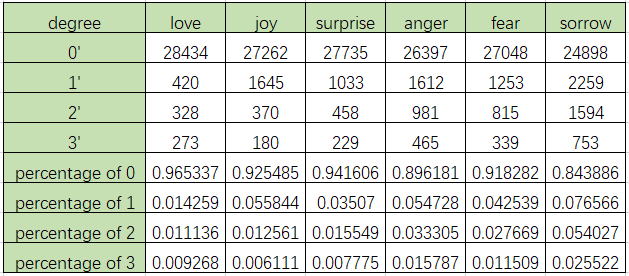
\includegraphics[scale=0.25]{data distribution.jpg}\\

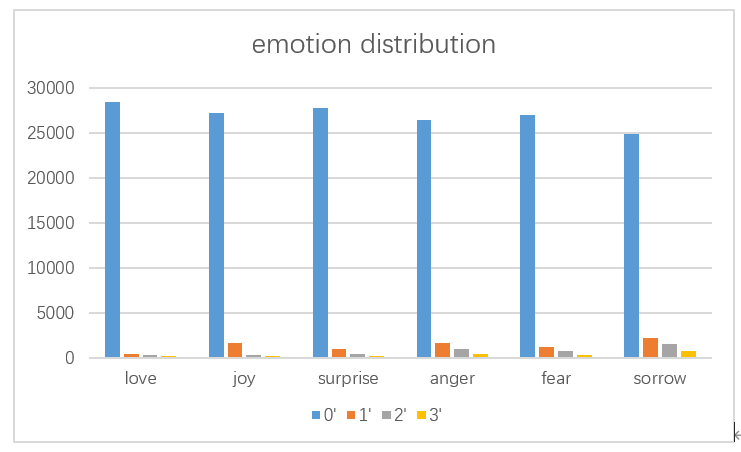
\includegraphics[scale=0.3]{emotion distribution.png}

%---------------------------------------------

\section{Our Work}

This is a part to show what we have done. Including:
\begin{enumerate}
\item Preparation work (study papers, tools, libraries).

\item Build the program environment.

\item Our baseline results.
\end{enumerate}

\subsection{Method}

This part includes the methods we use in the project. 

Our algorithm, including how to process the data, and turns to the problem of multi-label dichotomies of sentences.

Here is the description of our four methods.

\begin{enumerate}
\item Method 1

We implemented the baseline version using the simplest way and got a score of 0.6814 on the test set and 0.6787680571339884 on the validation set.

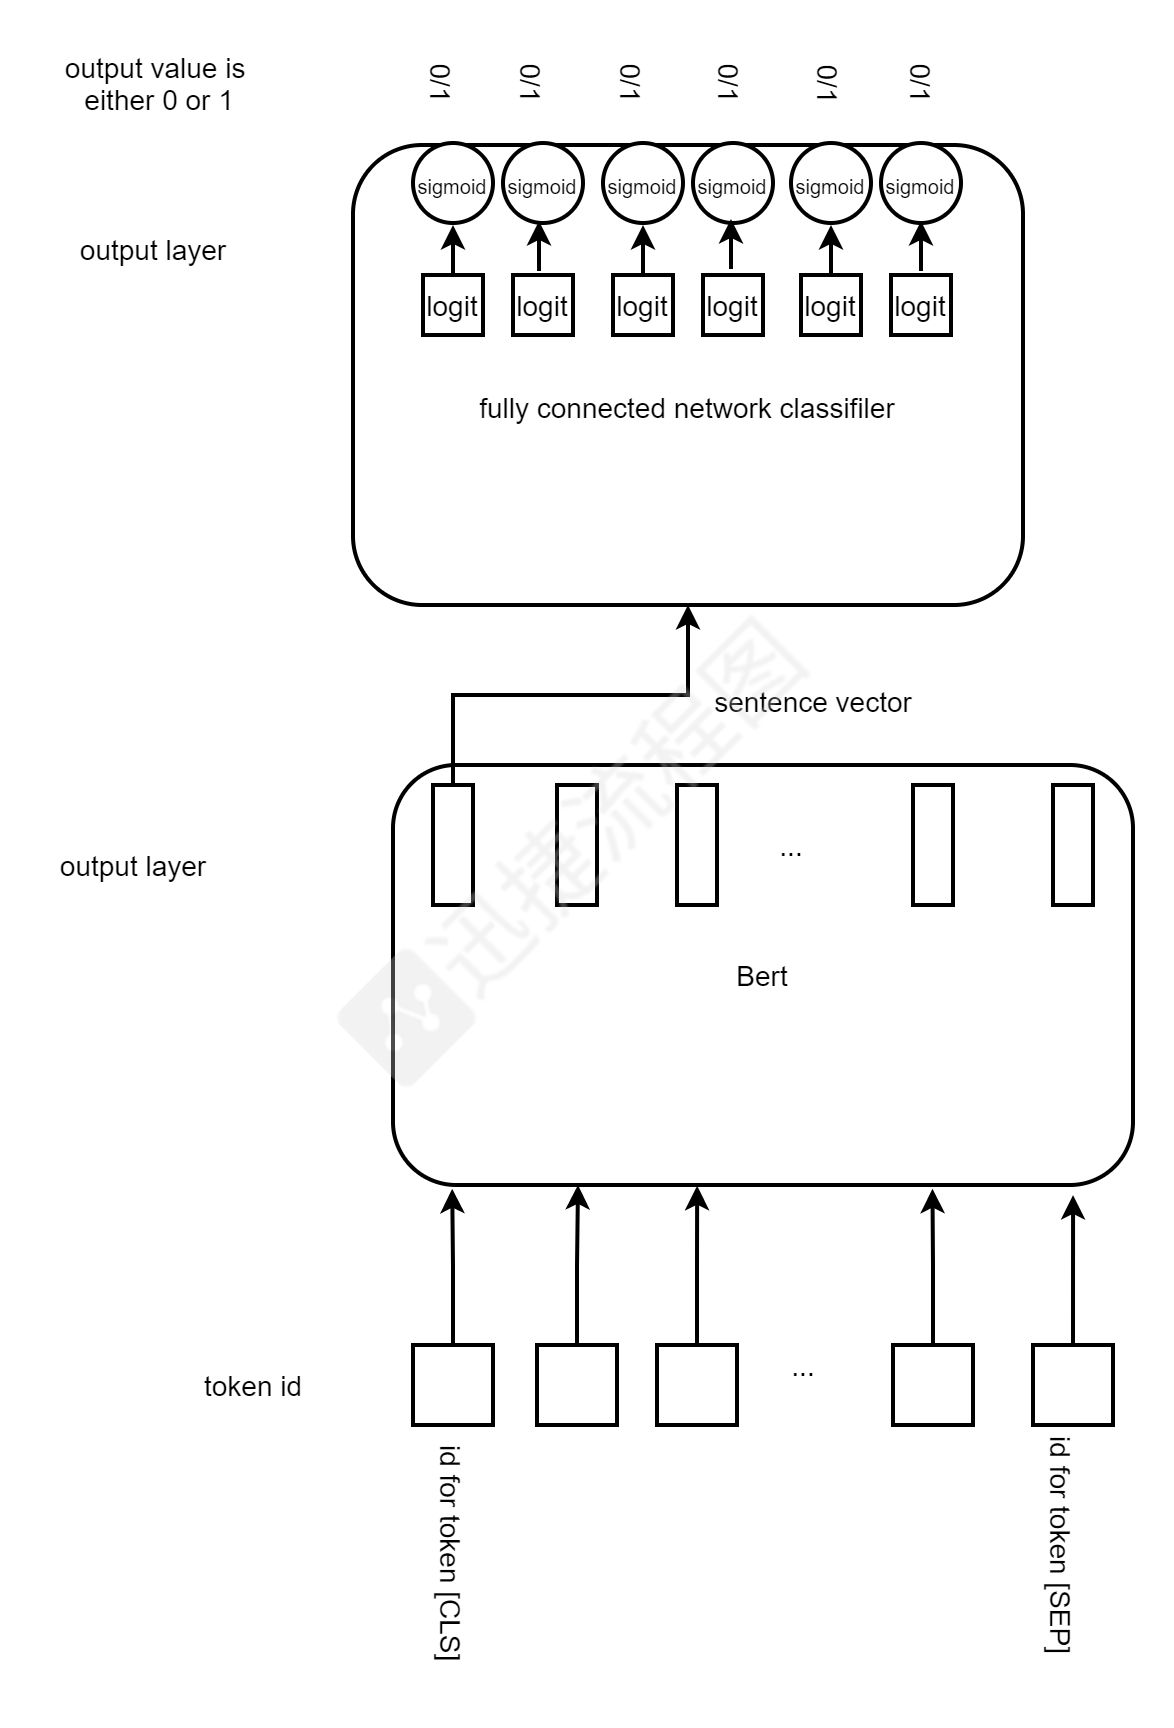
\includegraphics[scale=0.22]{Method1.png}

The method is described as below: 
\begin{enumerate}
\item By combining character names and dialogues into one text, the emotion recognition of the role becomes a text classification problem. Since there are multiple emotions to be recognized, it is a multi-label classification problem. The category of each label has four values [0,1,2,3]. However, from the perspective of data distribution, category 2 and 3 account for a relatively small proportion. In order to simplify, multi-label dichotomy is adopted. 
\item Scramble the data and divide it into training set and verification set in 8:2 ratio.  
\item The difference between multi-label classification and multi-label classification lies in:  

\begin{enumerate}
\item Multi-label classification refers to the classification of multiple aspects or targets of a sample, usually dichotomies. These aspects are not mutually exclusive. For example, for a sample picture of a person, it is male or female in terms of gender, adult or child in terms of age. These aspects of the image can occur simultaneously, both gender and age.  
\item Multi-classification problem is to tell which category a sample belongs to, the value of category is more than 2. These categories are mutually exclusive meaning that if a sample belongs to category 1, it cannot belong to category 2 or category 3. For example, the task of face recognition is to classify faces into different people's faces.  
\end{enumerate}

\item Our task is multi-label classification, because a sentence needs to be classified from multiple non-exclusive aspects (love, joy, surprise, anger, fear and sorrow). For simplicity, we only classify it into category 0 or 1, while category 2 and 3 are treated as category 1.  
\item To convert text into a vector, we adopt Bert-Base vector, which is currently popular and has good effects.  
\begin{enumerate}
\item We take a batch of text samples with a batch size of 8, calculate the maximum text length max-length-Batch of this batch of data, convert each character of the text into character ID first, and transform a batch of text padding of different lengths into the sequence of max\_length\_Batch of fixed length. Padding value is 0.  
\item Input the character ID sequence of the sample into Bert model, then extract the vector from the $0^{th}$ unit of the last layer of the Bert model as the vector of the whole sentence.  
\end{enumerate}
\item Send the sentence vector obtained into the fully-connected network for classification. Since there are six labels, the output is six neural units, and six logits are obtained.  
\begin{enumerate}
\item Different from the multi-classification, the multi-classification task is to put the six logits into Softmax, while the multi-label classification task is to put the six logits into sigmoid one by one, each value activated with sigmoid represents the probability which the tag is category 1.  
\item Convert labels with probability greater than 0.5 to 1, and labels with probability less than or equal to 0.5 to 0. 
\end{enumerate}
\item The loss function adopts binary cross-entropy.  

\item The flaws of Method 1:
\begin{enumerate}

\item In order to implement the task quickly, in Method 1, we use the ready-made toolkit Simpletransformer, we simplify the task and simplify the recognition of emotional value into multi-label dichotomization. In fact, there are four values of emotion: 0,1,2, and 3, which belong to multiple categories. 
Different from ordinary multiple categories, each category of this category is the intensity value of emotion, which is actually divided into different sizes. If it is regarded as a general classification problem, cross-entropy loss is adopted, then it cannot reflect the fact that the error between intensity value 1 and intensity value 3 is larger than the error between intensity value 1 and intensity value 2, so intuitively we think it makes more sense to turn to regression rather than categorization.  
\item Since emotion recognition is aimed at the designated role, the first method is simply to combine the characters of the role into the text of the script, so as to classify the text. But roles play a crucial role here, and if we combine them into text, we treat them like any other character in the text, which gives the model a chance to overlook the important role of roles.  
\item Through data analysis, we know that the emotional value is not only related to the current text, but also related to the plot above. The same sentence in different contexts will show different emotions, while Method 1 does not make use of the above information.  
\item Therefore, based on the above analysis, we gradually made improvements, thus gradually improving the scores of verification set and test set.    
\end{enumerate}
\end{enumerate}

\item Method 2

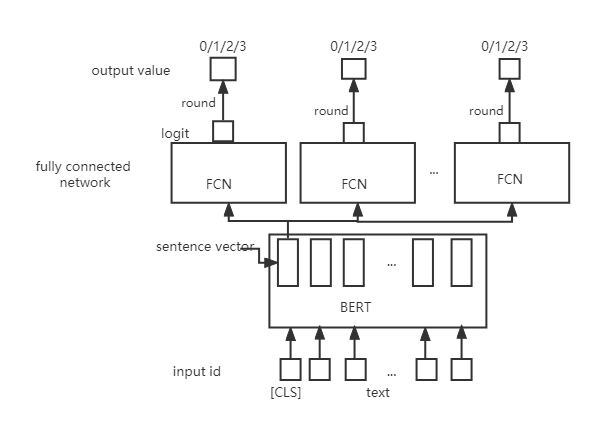
\includegraphics[scale=0.5]{Method2.png}

This is a classification method based on linear regression. We adopt multiple output blocks, one emotion corresponds to one output block, and there are two fully-connected networks inside each output block. The output dimension of the last layer is 1, without adding any activation function, logit is directly used as the output of linear regression, and the loss function is MSE. The resulting logit is a real number, and we round logit to get integers in the range [0,1,2,3]. The emotional values of the six emotions correspond to the integral values of the six output blocks. Since there are multiple output blocks, the total loss is the sum of the losses of all outputs. It's actually a multitasking approach to learning. Each task is to identify one of the emotions, but share sentence vectors. 

\item Method 3

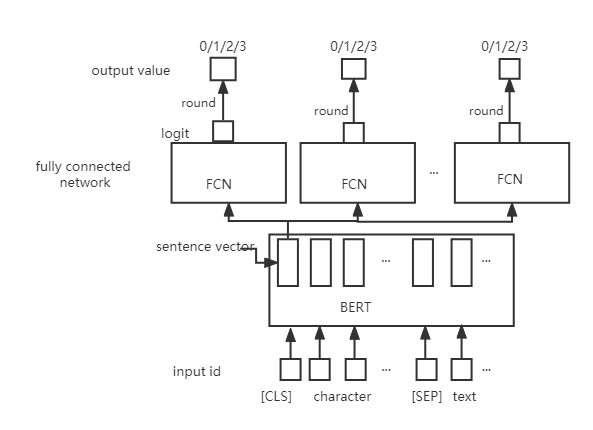
\includegraphics[scale=0.5]{Method3.png}

 On the basis of Method 2, we imitate the way BERT model handles question and answer task, taking character string as question Text 1 in question and text as reference text Text 2 in question and answer task. However, different from question and answer task, question and answer task classifies each character of sequence. To get the start and end of the answer in the text. Here we still take the vector from the $0^{th}$ position of the output layer as a vector representation of the text and the character, and this vector representation is processed as a feature input to the output block. Because Text 1 and Text 2 implement the attention mechanism within Bert, the model attaches much more importance to the role than Method 1 does.  

\item Method 4

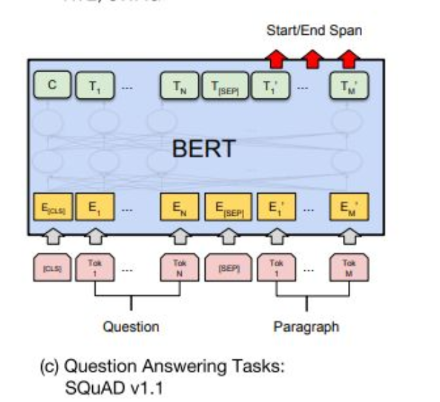
\includegraphics[scale=0.8]{bert1.png}\\

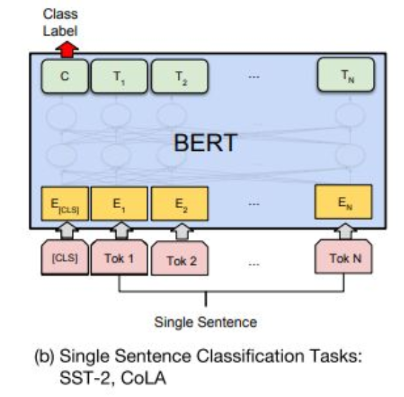
\includegraphics[scale=0.8]{bert2.png}\\

On the basis of Method 3, we introduce historical text. Due to the limited time, we only introduce the two sentences above for the time being, and simply merge the previous two sentences with the current text to get a larger text. In order to reference the historical text, we preprocess the data. We sorted the content in the script data according to the sequence of the story and de-numbered the content\_id as a script library. We find the content of the original training data and test data to content\_id, and then take the three corresponding texts of content\_id-2,content\_id-1 and content-id from the script library and merge them into one large text in sequence. 
In this way, we use historical text information to predict the character emotion of the current text. Since the text length of the model cannot be increased indefinitely, we only quote 2 sentences above for the time being. 


\item Our task is a multi-label classification, because a sentence needs to be classified from multiple non-exclusive aspects (love, joy, surprise, anger, fear, sorrow). For simplicity, we only classify it into category 0 or 1, while category 2 and 3 are treated as category 1.  

\item To convert text into vector, we use the current popular and better effect of Bert-Base vector.

\begin{enumerate}
\item We take a batch of text samples with a batch size of 8, calculate the maximum text length max-length-batch of this batch of data, convert each character of the text into character ID first, and transform a batch of text padding of different lengths into the sequence of max\_length\_batch of fixed length. Padding value is 0. 

\item Input the character ID sequence of the sample into the Bert model, and extract the vector from the $0^{th}$ unit of the last layer of the Bert model as the vector of the whole sentence.  
\item Send the sentence vector obtained into the fully connected network for classification. Since there are 6 labels, the output is 6 neural units, and 6 logits are obtained. 

\item Different from the multi-classification task, the multi-classification task is to make 6 logits as Softmax, while the multi-label classification task is to make 6 logits as sigmoid one by one, and each value activated with sigmoid represents the probability of this label as category 1.

\item Convert labels with probability greater than 0.5 to 1, and labels with probability less than or equal to 0.5 to 0.  



\end{enumerate}

\end{enumerate}


\subsection{Experiments}


\subsection{How to count the accuracy}

The score of the algorithm in this competition is calculated by the common root mean square error (RMSE), and the emotion values corresponding to the six emotions identified by "text content + character name" are counted:\\

$R M S E=\sqrt{\frac{\sum_{i=1}^{n} \sum_{j=1}^{6}\left(y_{i, j}-x_{i, j}\right)^{2}}{6 n}}$\\

score = 1/(1 + RMSE)\\

Where $y_{i,j}$ is the predicted emotion value, $x_{i,j}$ are the marked emotion value, and n is the total number of test samples.  
The final ranking is based on score.  

\subsection{Baseline score}

% 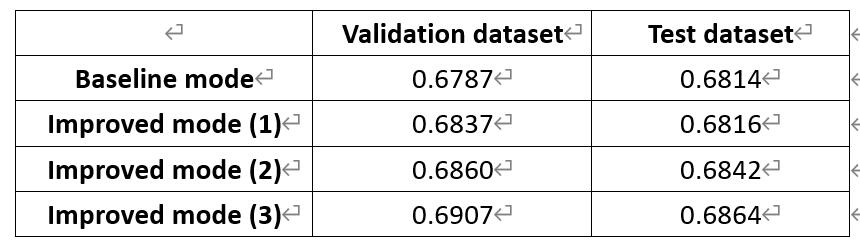
\includegraphics[scale=0.35]{bert3.jpg}\\
\newcommand{\tabincell}[2]{\begin{tabular}{@{}#1@{}}#2\end{tabular}}
\begin{tabular}{|c|c|c|} %l(left)居左显示 r(right)居右显示 c居中显示
\hline

Name & \tabincell{c}{Validation\\ Dataset} & \tabincell{c}{Test\\ Dataset}\\

\hline 
Baseline Model&0.6787&0.6814\\
\hline 
Improved Model (1)&0.6837&0.6816\\
\hline 
Improved Model (2)&0.6860&0.6842\\
\hline 
Improved Model (3)&0.6907&0.6864\\
\hline 

\end{tabular}
















%---------------------------------------------

\section{What remains to be done}

In the future, we plan to add a attention layer. After obtaining Bert sentence vectors for several sentences, they will be sent to the attention layer and the role vector for attention calculation to obtain sentence representations for longer texts, and then the output will be used for emotional value prediction.


Next steps:  
This network has an obvious disadvantage: first, the original multi-label and multi-classification task is simplified into multi-label dichotomy task, which reduces the performance of the model to a certain extent.  Second, the role to be identified is simply merged with the text, without explicitly telling the model which role the emotion to be identified is.  Third, the emotional values of the characters depend not only on the current text, but sometimes also on the historical text, and the network does not use historical information for prediction.  
Our next step is to try to implement a multi-label multi-classification network.  Since the category of classification has the relationship of degree and magnitude, we treat the classification problem as a regression problem, get the real value from 0 to 3, and then round it into an integer in {0,1,2,3}, so as to get the classification result.  
 
In the next step, we will refer to the question and answer task, regard the role as query, and conduct attention with text, so as to clearly tell the model which role's emotional value needs to be predicted.  




%-------------------------------------------------------------------------

   \makeatletter
    \renewcommand\@biblabel[1]{}
    \renewenvironment{thebibliography}[1]
    {\section*{\refname}%
    \@mkboth{\MakeUppercase\refname}{\MakeUppercase\refname}%
    \list{\@biblabel{\@arabic\c@enumiv}}%
    {\settowidth\labelwidth{\@biblabel{#1}}%
    \leftmargin\labelwidth
    \advance\leftmargin\labelsep
    \advance\leftmargin by 2em%
    \itemindent -2em%
    \@openbib@code
    \usecounter{enumiv}%
    \let\p@enumiv\@empty
    \renewcommand\theenumiv{\@arabic\c@enumiv}}%
    \sloppy
    \clubpenalty4000
    \@clubpenalty \clubpenalty
    \widowpenalty4000%
    \sfcode`\.\@m}
    {\def\@noitemerr
    {\@latex@warning{Empty `thebibliography' environment}}%
    \endlist}
    \makeatother

\begin{thebibliography}{99} 
\begin{enumerate}
\bibitem{Ref1}
% Format for Journal Reference
Dorottya Demszky, Dana Movshovitz-Attias, Jeongwoo Ko,Alan Cowen, Gaurav Nemade, Sujith Ravi:  GoEmotions: A Dataset of Fine-Grained Emotions
\bibitem{Ref2}
Wenhao Ying, Rong Xiang, Qin Lu: Improving Multi-label Emotion Classification by Integrating both General and Domain Knowledge
\bibitem{Ref3}
Lei Zhang, Shuai Wang, Bing Liu: Deep Learning for Sentiment Analysis: A Survey

\bibitem{Ref4}
Devlin J,Chang MingWei,Lee K,et al. BERT:Pretraining of deep bidirectional transformers for language understanding[C] // Proceedings of the 2019 Conference of the North American Chapter of the Association for Computational Linguistics:Human Language Technologies. Minneapolis,USA,2019:4171-4186

\bibitem{Ref5}
Ashish V,Noam S,Niki P,et al. Attention is all you
need[C]// Proceedings of the $30^{th}$ International Conference on Neural Information Processing Systems. Long Beach,USA,2017:5998-6008

\end{enumerate}
\end{thebibliography}


\end{document}
